\chapter{0次ホールドされた正弦波の周波数特性}
    \label{0次ホールドされた正弦波の周波数特性}
    \section{背景}
        既に述べたように、信号処理や制御工学では実用上、入力と制御対象の間に0次ホールド回路と演算回路が挟まった形になる。
        技術書の中にはこれをステップ入力に対するラプラス変換の積分と時間遅れとして表してゲインや位相を考えているものもあるが、これは厳密には正しくない。
        なぜなら、0次ホールド回路に正弦波を入れた際、通過した信号は細かいステップの集まりであり、元の正弦波に近いものの、完全な正弦波ではないからである。
        「ゲイン」や「位相変化」を厳密に定義できない。
        厳密には、Fourier変換してスペクトラムについて考える必要がある。
        とはいえ、無限に続く減衰しない信号のFourier変換は通常の関数の意味では存在しないし(超関数になる)、現実の測定器は窓関数で時間制限した信号のFourier変換を近似的に計算している。
        そこで本記事では窓関数付きのFourier変換の結果ついて考察する。
    \section{導出}
        $f_0>0$とし、連続時間の複素正弦波信号$x:t\in\realNumbers\mapsto\exp(i 2\pi f_0 t)$を考える。
        サンプリング周期を$\Ts>0$とする。
        この周期で$x$を0次ホールドした信号を$\xd:t\in\realNumbers\mapsto x(\floor{t/\Ts}\Ts)$とする。
        次の図は$x$と$\xd$の実部を示したものである。
        \begin{figure}[H]
            \centering
            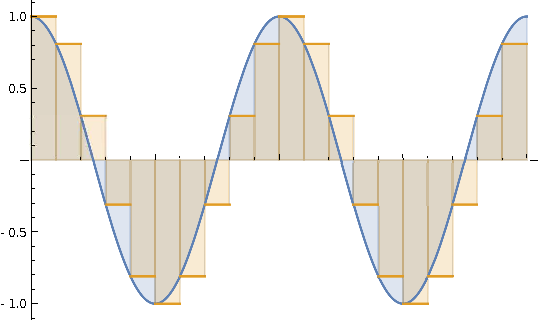
\includegraphics[keepaspectratio, scale=0.6]
            {\currfiledir/imgs/0-order-held-sinusoid.pdf}
            \caption{元の信号とその0次ホールド}
        \end{figure}
        上の図より、$\xd$の基本周波数成分(周波数成分に於ける$f_0$に対応する成分)が$x$のそれより遅れることが予想される。
        このことを矩形窓を通した、周波数表示されたFourier変換で考察する。
        $N\in\naturalNumbers$とし、窓の幅を$T=N\Ts$とする。
        窓の幅を$\Ts$の整数倍に選んでいるが、非整数倍の場合でも幅を十分に大きくとれば小数部分に対応する区間の積分の$1/T$倍は無視できるほど小さくなり、最も近い整数倍の幅を用いた結果と殆ど一致する。
        $x$の窓付きFourier変換を窓の幅で規格化したものは次式である。
        \[ X(f) = \frac{1}{T} \integrate{0}{T}{x(t)\exp(-i 2\pi f t)}{}{t} = \frac{1}{i 2\pi(f-f_0)T}\left(1-\exp\left(-i 2\pi(f-f_0)T\right)\right) \]
        $\xd$の窓付きFourier変換は次式である。
        \begin{align*}
            \Xd(f) &= \frac{1}{T}\integrate{0}{T}{\xd(t)\exp(-i 2\pi f t)}{}{t} = \frac{1}{T}\sum_{k=0}^{N-1}\integrate{k\Ts}{(k+1)\Ts}{\xd(t)\exp(-i 2\pi f t)}{}{t} \\
            &= \frac{1}{T}\sum_{k=0}^{N-1}\exp(i 2\pi f_0 k\Ts)\integrate{k\Ts}{(k+1)\Ts}{\exp(-i 2\pi f t)}{}{t} \\
            &= \frac{1}{T}\sum_{k=0}^{N-1}\exp(i 2\pi f_0 k\Ts)\frac{1}{i 2\pi f}\exp(-i 2\pi f k\Ts)\left(1-\exp(-i 2\pi f \Ts)\right) \\
            &= \frac{1-\exp(-i 2\pi f\Ts)}{i 2\pi f}\frac{1}{T}\underbrace{\sum_{k=0}^{N-1}\exp(i 2\pi(f_0-f)k\Ts)}_{\text{(A)}} \\
            &= \frac{1-\exp(-i 2\pi f\Ts)}{i 2\pi f}\frac{1}{N\Ts}\exp(i\pi(f_0-f)(N-1)\Ts)\frac{\sin\pi(f-f_0)N\Ts}{\sin\pi(f-f_0)\Ts}
        \end{align*}
        最後の式を導くために、(A)に等比数列の和の公式を適用し、分母・分子それぞれ$\sin$が生じるように複素指数関数を括り出して整理した。
        \par
        $\xd$中の、周波数が$f_0$である成分の振幅と位相を調べる。
        $f\to f_0$の極限に関して次式が成り立つ。
        \[ \lim_{f\to f_0} \Xd(f) = \frac{1-\exp(-i 2\pi f_0\Ts)}{i 2\pi f_0\Ts} \]
        これより、上式に相当する振幅と位相の変化が生じる。
        サンプリングが十分に高速、すなわち$f_0\Ts\ll 1$であるとき上式は1に近づくので、振幅と位相の変化は無くなってゆく。
        \par
        次に、高調波領域を調べる。
        $|\Xd(f)|$は$1/\Ts$周期関数と$1/|f|$の積であるので、$|f|<\Ts/2$の部分の縮小コピーが高周波領域に於いて$1/\Ts$毎に現れる。
        これが高調波成分である。
    \section{数値例}
        今、$f_0=10,\;\Ts=10^{-2},\;N=200$とする。
        $f=f_0$に於ける振幅と位相は$|\Xd(f_0)| \approx 0.9836,\quad \angle \Xd(f_0) \approx \ang{-18.00}$となる。
        次の図は$f_0$近傍でのパワースペクトル$X,\Xd$を示したものである。
        \begin{figure}[H]
            \centering
            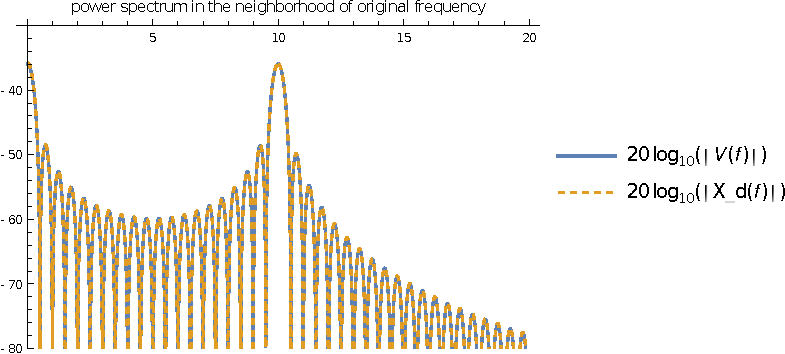
\includegraphics[keepaspectratio, scale=0.8]
            {\currfiledir/imgs/spectrum_in_the_neighborhood_of_original_frequency.pdf}
            \caption{元の周波数の近傍でのパワースペクトル}
        \end{figure}
        低周波領域では両者が良く一致していることがわかる。
        \par
        次に高調波を見る。
        次の図はサンプリング周波数の3倍の範囲まで$X,\Xd$を示したものである。
        \begin{figure}[H]
            \centering
            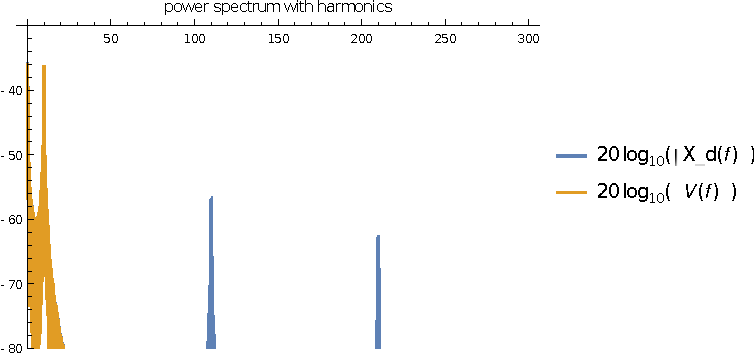
\includegraphics[keepaspectratio, scale=0.8]
            {\currfiledir/imgs/power_spectrum_with_harmonics.pdf}
            \caption{高調波を含むパワースペクトル}
        \end{figure}
        サンプリング周波数の整数倍の位置に高調波が生じていることが判る。
        \par
        この数値例を計算したMathematicaノートブックおよびMATLABスクリプトは下記のファイル名で保存されている。
        Gitリポジトリ内でファイル名検索すれば発見できるであろう。
        \begin{itemize}
            \item \href{\currfiledir/spectrum_of_zero-order-held-sine-wave.nb}{spectrum\_of\_zero\-order\-held\-sine\-wave.nb}
            \item \href{\currfiledir/spectrum_of_zero_order_held_sine_wave.m}{spectrum\_of\_zero\_order\_held\_sine\_wave.m}
        \end{itemize}